\begin{figure}[H]
\centering
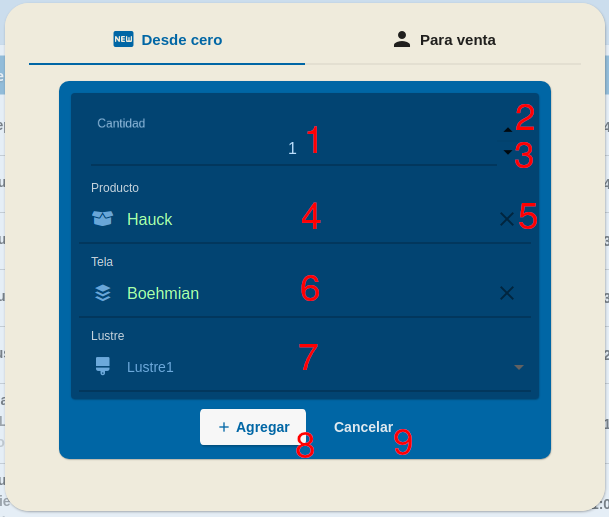
\includegraphics[width=\textwidth,height=\textheight,keepaspectratio]{Escenarios/AD-24-00}
\caption{Escenario - AD-24-00}
\label{fig:AD-24-00}
\end{figure}

Este escenario permite a un usuario crear/modificar una linea de orden de producción, en caso de estar modificando los campos estarán autocompletados con la información actual de la linea de orden de producción, pudiendo modificarlos. En el campo \textbf{AD-24-01} se debe ingresar la cantidad a producir, pudiendo incrementar y decrementar dicha cantidad con los botónes \textbf{AD-26-02} y \textbf{AD-24-03}. En el campo \textbf{AD-24-04} se debe ingresar un producto, este campo cuenta con el botón \textbf{AD-24-05} el cual permite borrar el texto ingresado. El campo \textbf{AD-24-06} permite seleccionar una tela y la lista desplegable \textbf{AD-24-07} permite indicar un lustre. El botón \textbf{AD-24-08} agregará o modificará la linea de orden de producción según corresponda indicando en el mismo: 'Agregar' con el icono \faTimes , o 'Modificar' con el icono \faEdit. 
El botón \textbf{AD-24-09} permite cancelar la operación, navegando al escenario \textbf{AD-23-00}.
\clearpage
